\documentclass{scrartcl}
\usepackage[ngerman]{babel}
\usepackage[utf8]{inputenc}
\usepackage{graphicx}
\usepackage[T1]{fontenc}
\usepackage{soulutf8}
\usepackage{hyperref}
\usepackage{rotating}
\usepackage{geometry}
\usepackage{float}


\begin{document}

\begin{titlepage}
\thispagestyle{empty}
\titlehead{\centering Designdokument}
\title{Reliable Computing on a \textbf{Fa}ult \textbf{T}olerant \textbf{Net}work in Space (FaTNet)\bigskip}
\subtitle{\bigskip $\;$ \bigskip Studentisches Projekt am deutschen Zentrum für Luft- und Raumfahrt e.V. (DLR)}
\bigskip

\author{Wintersemester 2012/2013 bis Sommersemester 2013\bigskip}
\date{\bigskip}
\publishers{Bearbeitet von:\\Andre Pols, Christian Uphaus, David Weigel, Esther Funken, Gerfried Oltmanns, Jonas Rahlf, Simon Schaller, Stefan Rasch, Tobias Sachtje\\ \bigskip \vspace*{10mm} \today \\ \bigskip \vspace*{10mm} Version: 2.1}
\begingroup
 \makeatletter
 \@titlepagetrue
 \maketitle
\endgroup
  %\newpage
\end{titlepage}

\pagenumbering{roman}

\newpage
\tableofcontents
\clearpage
\pagenumbering{arabic}
\section{Einleitung}
\label{Einleitung}
Das Projekt „Reliable Computing on a Fault Tolerant Network in Space” (kurz: FatNet) ist im Rahmen des Systemtechnikprojekts für Studierende des Studiengangs Systems Engineering ausgeschrieben. Es soll ein zuverlässiges und fehlertolerantes System entwickelt werden. FaTNet basiert auf der Problematik, dass im Weltraum auftretende, technische Ausfälle in den meisten Fällen nicht behoben werden können. Deshalb ist beim Systementwurf darauf zu achten eben diese Ausfälle kompensieren zu können.
Das Projekt wird von Görschwin Fey, Fabian Greif und Carl Johann Treudler betreut.
Es nehmen folgende Studenten an dem Projekt teil: Andre Pols, Christian Uphaus, David Weigel, Esther Funken, Gerfried Oltmanns, Jonas Rahlf, Simon Schaller, Stefan Rasch und Tobias Sachtje.
\section{Laufzeit und Organisation}
\label{LauzeitUndOrganisation} 
Das Projekt beginnt im Wintersemester 2012 (15.10.2012) und hat eine Laufzeit von zwei Semestern.

Während der gesamten Laufzeit sind die Projektmitglieder selbst für ihren Fortschritt zuständig. Zwei der Projektmitglieder werden zu Anfang bestimmt, um sich fortan um allgemeine organisatorische Inhalte zu kümmern.
   
Da jedes Mitglied andere Kompetenzen und Interessen vorzuweisen hat, kann in erster Linie jeder selbst bestimmen, an welchen Teilprojekten er/sie mitarbeiten möchte. Dazu werden Arbeitspakete definiert und Personen zugeordnet.
   
Des weiteren gibt es ein wöchentliches Gesamtgruppentreffen, um alle Arbeiten der Woche vorzustellen und das weitere Vorgehen gemeinsam zu planen. Diejenigen Mitglieder, welche zu spät oder gar nicht erscheinen, haben sich vorher abzumelden. Zusätzlich findet regelmäßig ein Treffen mit den Betreuern statt.

Damit alle Projektteilnehmer auf dem Laufenden bleiben, ist ein Projektverwaltungstool (FB3 Redmine) eingerichtet, das ein Wiki, ein Versionsverwaltungssystem sowie eine Ablage für Dokumente und Gantt-Diagramme bereitstellt. Dort findet sich auch das Dokument Arbeitsablauf.vsd in welchem die Arbeitspakete, die Verantwortlichen und die geschätzte Bearbeitungszeit eingetragen sind.

\section{Projektziel}
\label{Projektziel}
Das Projektziel ist es, ein fehlertolerantes System zu entwerfen, zu bauen und dieses zu präsentieren.
Zur Veranschaulichung der Fehlertoleranz wird ein Demonstrationssystem (im folgenden Demonstrator genannt) entworfen, in welches Fehler injiziert und anschließend von diesem behandelt werden.
Dabei sei angemerkt, dass das System nicht gegen jeden Fehler tolerant ist, sondern nur gegen diejenigen, die für die Demonstration eingeplant werden.
Die Gestaltung des Systems wird anhand seines Missionszieles durchgeführt.

Folgende abstrakte Fehler sollen im Rahmen der Fehlertoleranz kompensiert werden können:

\begin{itemize}
	\item Teilausfall der Kommunikation
	\item Ausfall von Motoren
	\item Ausfal/St"orung von optischen Sensoren
	\item Ausfall von anderen Sensoren
	\item Ausfall von Mikrocontrollern mit unterschiedlichen Aufgaben
\end{itemize}

%Diese Fehler wurden nach den folgenden Kriterien ausgesucht:

%\begin{itemize}
%	\item Darstellbarkeit
%	\item Plausibilität
%	\item Injizierbarkeit
%	\item Auswirkung
%	\item Behhebarkeit
%\end{itemize}

Ein Ausfall bedeutet das die betroffene Komponente vollst"andig inaktiv ist, eine St"orung bedeutet das die Komponente falsche Daten liefert.  
Alle Fehler können tatsächlich auftreten, lassen sich leicht und anschaulich injizieren und haben eine angemessene Auswirkung auf das System.
\section{Mission}
\label{Mission}
Die Mission beschreibt die Aufgaben und Zielsetzungen des Systems die vom Projektziel abgeleitet sind.
Das System hat die Mission sich in einem durch Wände abgetrennten Raum mit ebenem Boden autonom zu bewegen. Dabei sucht das System nach einem definierten visuellen Signal (farbig) an den Wänden des Raumes. Hat das System ein solches Signal gefunden, benutzt es seinen Manipulator um mit diesem Signal zu interagieren.\\
Diese Mission muss vom System in unterschiedlichen Stufen von Komponentenversagen so gut es geht in mehreren Testläufen durchgeführt werden.\\
\section{Systementwurf}
\label{Systementwurf}
Aus dem Projekt- und Missionsziel leiten sich die folgenden Anforderungen an das System ab.
Um sein Missionsziel zu erfüllen muss sich der Demonstrator bewegen können. Hierfür besitzt er mehrere Antriebsmotoren. Um sein Umfeld wahrzunehmen und das Zielsignal zu erkennen benötigt er Kameras und Abstandssensorik. Außerdem benötigt das System einen Manipulator mit drei Freiheitsgraden um nur durch den Manipulator in allen drei Raumrichtungen mit dem Ziel zu interagieren.
Den Kern des Systems bilden drei STM-32 Mikroprozessoren, die über zwei CAN-Busse miteinander kommunizieren. Zusätzlich zu den Mikroprozessoren hängt noch ein Monitor an den Bussen, der entscheidet welcher Mikroprozessor die Antriebsmotoren über H-Brücken ansteuert.

Im  Blockschaltbild (Abbildung 1) sind alle Grundlegenden Elemente der Hardware und deren Verknüpfung miteinander aufgezeigt.
\begin{figure}[H]
\centering
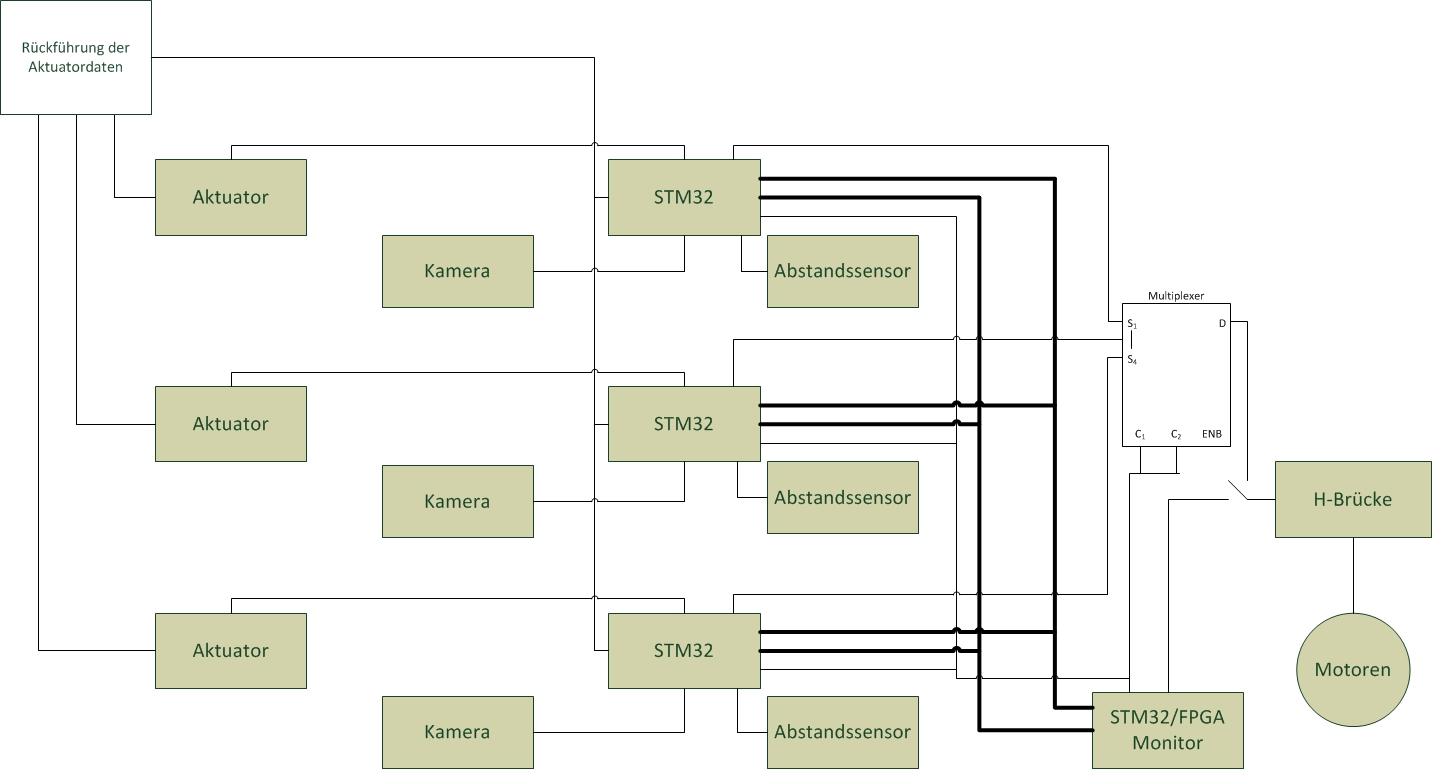
\includegraphics[width=1\linewidth]{Bilder/FaTNet_blockdiagramm.jpg}
\caption{Verknüpfung der Hardware-Elemente} 
\end{figure}
Jeder Mikroprozessor ist für eine Kamera und einen Abstandssensor zuständig und bearbeitet deren Daten. Zusätzlich steuert jeder Mikroprozessor einen Motor des Manipulators und ist somit für einen Freiheitsgrad zuständig. Damit das System unter bestimmten Bedingungen, welche die Freiheitsgrade einschränken, sein Missionsziel noch so gut wie möglich erfüllen kann, hat jeder Mikroprozessor Kenntnis über die Position aller Aktuatoren. Das System ist dadurch in der Lage wegfallende Freiheitsgrade zu kompensieren.

\subsection{Mechanik}
\label{SystementwurfMechanik}
Die Abbildung 2 zeigt die funktionalen Bauteile und deren schematische Anordnung.
Dieser Anordnung zeigt au"serdem die allgemeine Gestalt des Demonstrators, die genauen geometrischen Dimensionen sind noch nicht festgelegt :
\begin{figure}[H]
\centering
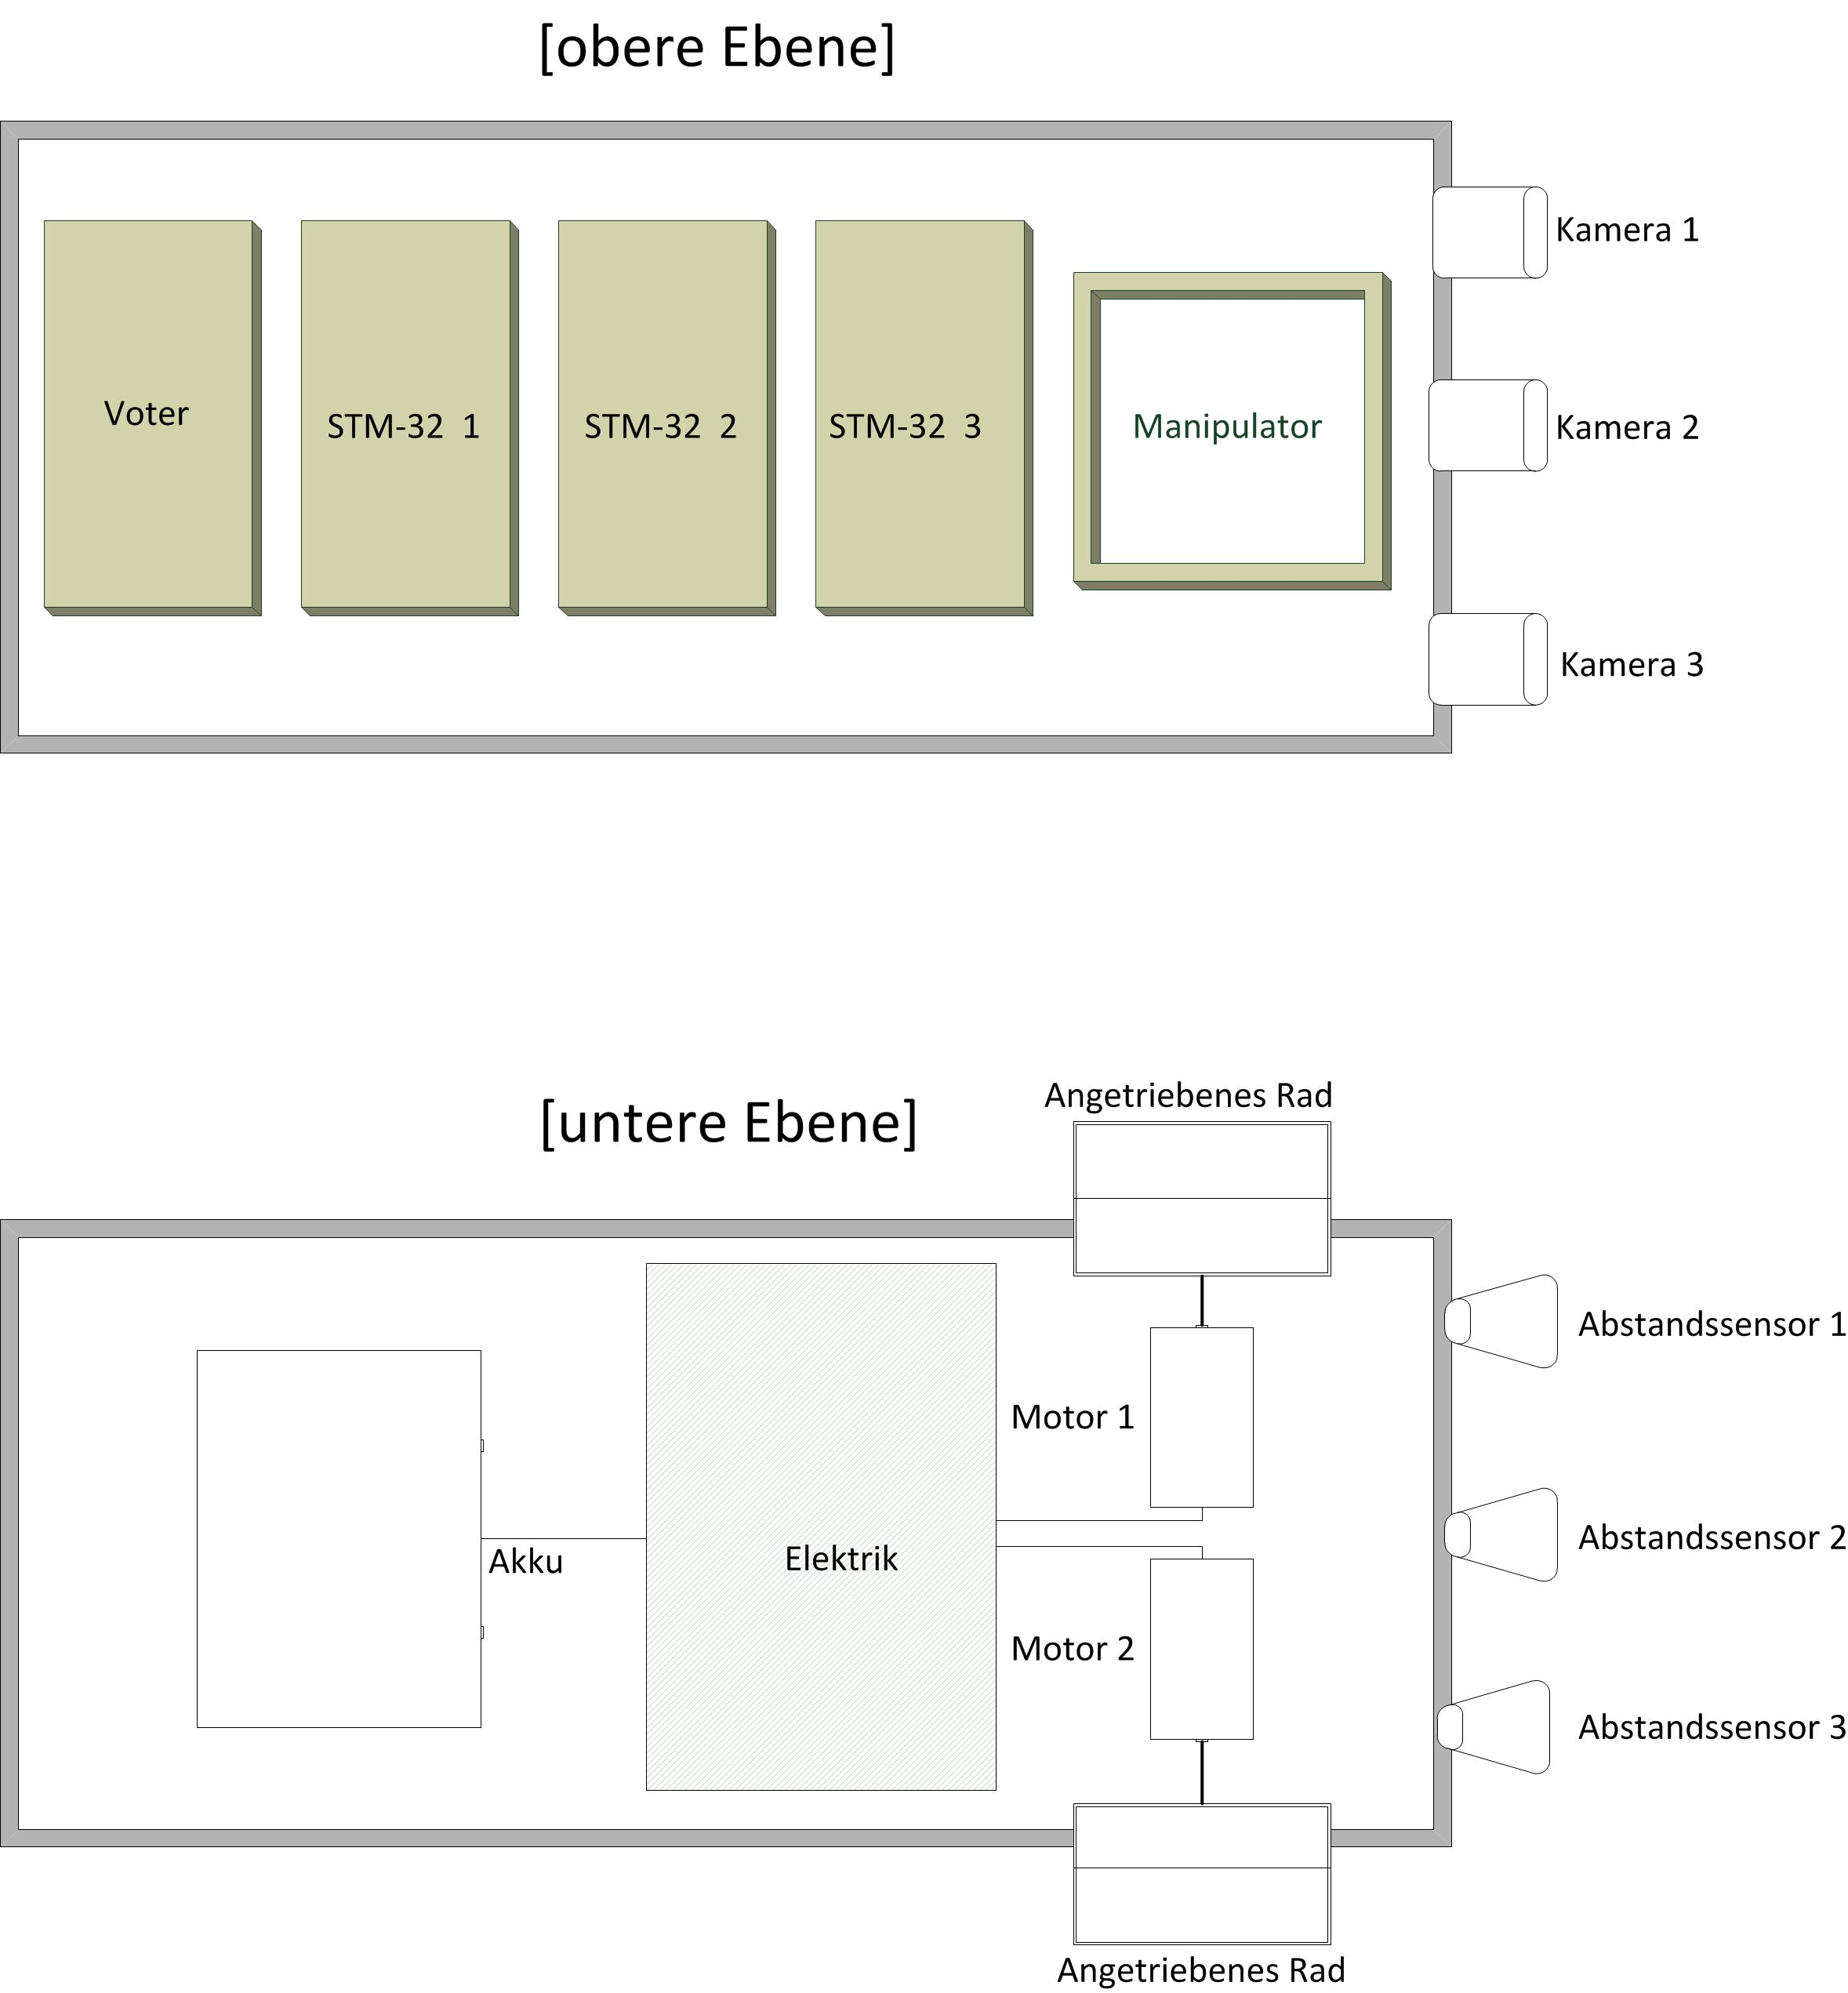
\includegraphics[width=0.7\linewidth]{Bilder/FaTNet_mechanik}
\caption{Anordnung der Komponenten}
\end{figure}
Das Layout der Komponenten ist so vorgesehen, dass alle Elemente auf zwei Ebenen liegen. Würde alternativ jedes STM auf einer separaten Plattform platziert sein oder diese senkrecht aufgestellt werden, wäre es während der Demonstration einerseits schwerer die Fehler am fahrenden System zu injizieren und andererseits wäre nicht genau zu erkennen, welche Fehler injiziert werden.

\subsubsection{Manipulator}
\label{kap:Manipulator}
Am Manipulator sollen die Fehler durch “Graceful degradation” behandelt werden.
Dies bedeutet, dass im Fehlerfall die betroffene Komponente abgeschaltet wird und der Funktionsumfang reduziert wird. Dabei ragt das interagierende Ende in jedem Fall über das Chassis hinaus, so dass, selbst wenn alle Aktuatoren ausfallen, der Arm noch benutzt werden kann.
Fällt nur ein Freiheitsgrad weg, so kann dieser zu einem gewissen Teil durch die Chassis-Konstruktion kompensiert werden:
Die Rotation um die vertikale Achse kann zu einem gewissen Teil durch die Positionierung des Systems ausgeglichen werden.
Fällt ein Aktuator der horizontalen Achse aus wird die Reichweite des Armes eingeschränkt, kann aber durch den zweiten Aktuator in Verbindung mit der Position des Systems ausgeglichen werden.
\begin{figure}[H]
\centering
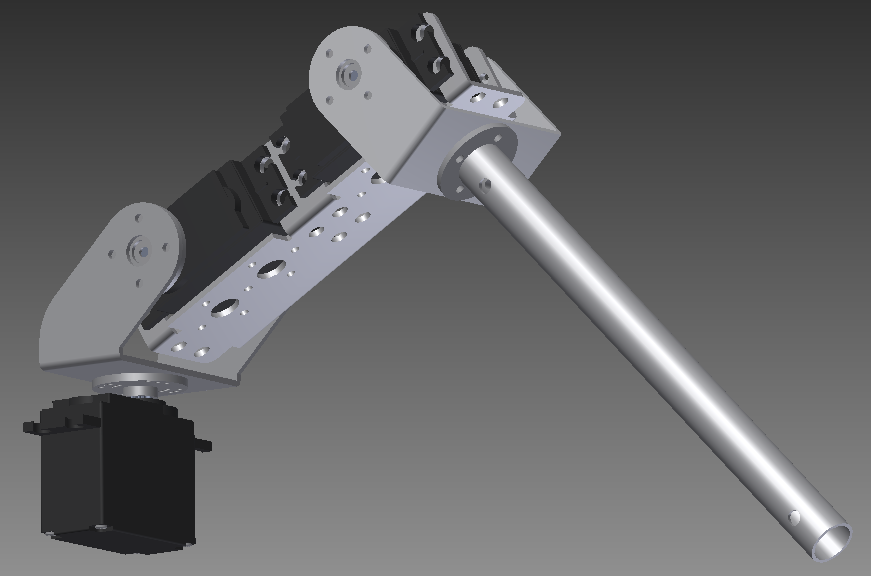
\includegraphics[width=0.5\linewidth]{Bilder/FaTNet_manipulator}
\caption{3D-Entwurf eines Manipulators}
\end{figure}

\subsection{Systementwurf Elektronik}
\label{SystementwurfElektronik}

\subsubsection{Elektrische Leistung}
Die folgende Tabelle zeigt die Komponenten auf, die elektrisch versorgt werden müssen. Die Werte, welche unter Watt eingetragen sind, sind die Worst-Case beötigten Versorgungsleistungen. Unter Umständen wird ein LC-Display benötigt, dahe rwird es mit aufgeführt. Unter Anzahl ist angegeben wieviele dieser Komponenten maximal im System verbaut werden.
Sind konkrete Komponenten angegeben so handelt es sich um Vorschläge die im Rahmen dieser Überschlagsrechnung Sinn ergeben.
\begin{table}[H]
\centering
\begin{tabular}{|c|c|c|}
\hline 
\textbf{Verbraucher} & \textbf{Maximale Leistungsaufnahme in Watt} & \textbf{Anzahl} \\ 
\hline 
Motor & 17 & 2 \\ 
\hline 
Mikrocontroller & 2.5 & 4 \\ 
\hline 
Kamera (OV7670) & 0.06 & 3 \\ 
\hline 
Display & 0.056 & 3 \\ 
\hline 
Servomotor & 2.7 & 4 \\ 
\hline 
\end{tabular}
\caption{Abschätzung des Leistungsbedarfs der Elektronik-Komponenten}
\label{tab:leistung}
\end{table} 
In der Summe ergibt sich ein Leistungsbedarf von rund 53 Watt. Eine Laufzeit von einer Stunde wird als erstrebenswert angesehen. Daraus resultiert eine benötigte Energiemenge von 53 Wattstunden.

\subsubsection{Energiespeicher}
Es werden LiFePo4-Akkumulatoren als Energiequelle verwendet werden.
%Ein Akku aus drei Zellen (11,1 Volt Nennspannung) müsste eine Kapazität von 4,8 Amperestunden besitzen, um die oben %aufgestellte Laufzeitanforderung zu erfüllen. Bei einem vierzelligen Akku (14,8 V) wären es 3,6 Amperestunden.

\subsection{Software}
Im folgenden Abschnitt wird grob auf die Softwarearchitektur eingegangen. Es wird erklärt, wie sich das System nach dem Einschalten verhält, an welcher Stelle die essentiellen Aktionen ausgeführt werden und an welchen Stellen dabei Fehler auftreten können. Von der Beschreibung der jeweils unterliegenden Algorithmen wird an dieser Stelle abgesehen.
Die Programmierung der verwendeten STM32-Mikrocontroller erfolgt in C++. Dabei wird auf die XPCC-Library (Cross Platform Component Communication) zurückgegriffen.

\subsubsection{Grundstruktur}
Nachdem der Mikrocontroller mit Spannung versorgt wird und gebootet ist, wird mit der Initialisierung der einzelnen Softwaremodule begonnen. Geplant sind folgende Module: 
\paragraph{CAN-Bus und  Protokoll}$\;$\\
Dieses Modul dient zur Kommunikation zwischen den verschiedenen STM-Boards. Dabei bildet der CAN-Bus das grundlegende Kommunikationsinterface. Auf dieses wird ein an der Problemstellung angepasstes Protokoll aufgesetzt. Eine funktionierende Kommunikation ist Voraussetzung um am Netzwerk teilzunehmen.

\paragraph{Heartbeat}$\;$\\
Durch den Heartbeat wird den übrigen Komponenten mitgeteilt, dass der Absender im Netzwerk zur Verfügung steht. Gegebenfalls können Fehler, die bei einem Teilnehmer auftreten, übermittelt werden. Ist es nicht möglich einen Heartbeat zu senden wird davon ausgegangen das keine Kommunikation vorhanden ist und es kommt zu einer  Fehlerbehandlung. Solange ein Heartbeat über das Netzwerk empfangen kann mit den Absender kommuniziert werden.

\paragraph{SysTick}$\;$\\
Der SysTick-Handler wird in fest definierten Zeitabständen per Interrupt aufgerufen. Im Handler werden Aufgaben ausgeführt die in regelmäßigen Abständen von Nöten sind. Beispielsweise die Regelung und der Heartbeat.

\paragraph{Kamera/Bildverarbeitung}$\;$\\
Die Kamera und die Verarbeitung der resultierenden Bilder wird zur Orientierung in der Umwelt verwendet. Nachdem die Informationen mittels Segmentierung, Klassifizierung und Positionbestimmung aus dem Bild extrahiert wurden, werden diese mit denen der anderen Teilnehmern verglichen um die Plausibilität zu prüfen. Die Informationen werden anschließend an den Wegplaner übergeben. Ist die Markierung in Reichweite wird von einer weiteren Wegplanung abgesehen. Stattdessen wird die Steuerung für den Roboterarm aufgerufen.

\paragraph{Abstandssensoren}$\;$\\
Dienen zur Vermeidung von Kollisionen. Deren Werte fließen ebenfalls in der Wegplanung mit ein.

\paragraph{Antrieb/ Regelung}$\;$\\
Die Regelung wird regelmäßig im SysTick-Handler ausgeführt. Die durch die Trajektorie vorgegebenen Soll-Werte werden mit den Ist-Werten der Encoder, welche die Drehzahl der Motoren zurückgeben, verglichen und gegebenfalls korrigiert. Der Voter legt in gleichmäßigen Zeitabständen einen Mikrocontroller als Master fest, der die Motoren regelt.

\paragraph{Roboterarm}$\;$\\
Befindet sich das System in der Position, dass der Manipulatior mit dem Ziel interagieren kann wird von der Wegplanung auf die Manipulatorsteuerung umgeschaltet. Die Winkelvorgabe der Aktuatoren geschieht per inverser Kinematik. Dabei müssen für den Ausfall von Aktuatoren mehrere Kinematik vorhanden sein, um das Ziel weiterhin zu erreichen.
 
\begin{figure}[H]
\centering
  \begin{minipage}[b]{0.49\linewidth}
    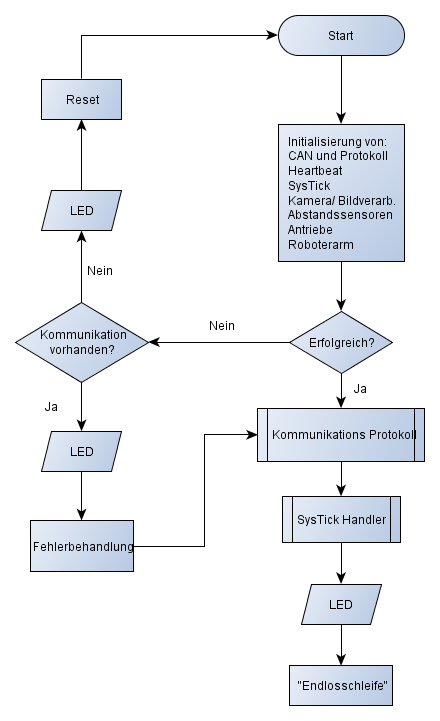
\includegraphics[width=\linewidth]{Bilder/FaTNet_init} 
    \caption{Flussdiagramm zur Initialisierung }
    \label{fig:init}
  \end{minipage}
  \begin{minipage}[b]{0.49\linewidth}
    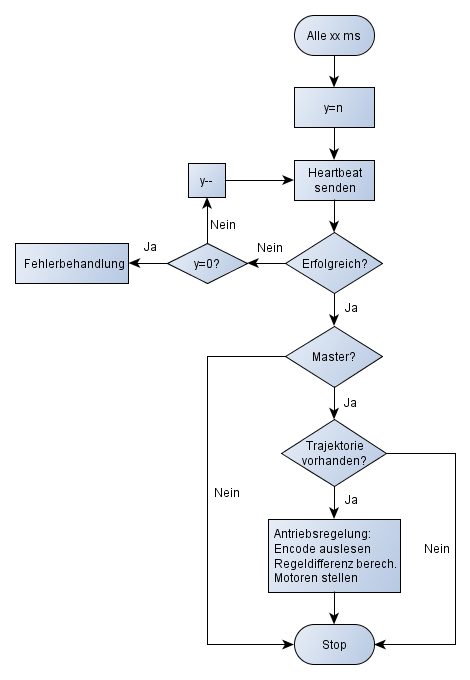
\includegraphics[width=\linewidth]{Bilder/FaTNet_systick}  
    \caption{Flussdiagramm zum SysTick-Handler}
    \label{fig:systick}
  \end{minipage}
\end{figure}

\begin{figure}[H]
\centering
    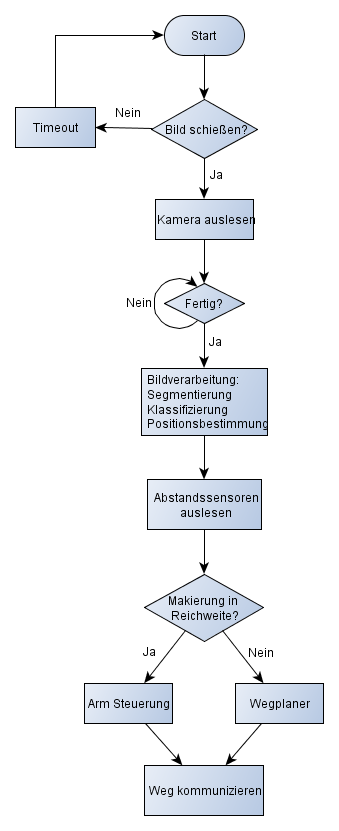
\includegraphics[width=0.4\linewidth]{Bilder/FaTNet_schleife}  
    \caption{Flussdiagramm zum Softwareablauf}
    \label{fig:schleife}
\end{figure}

\section{Fehlerverhalten}
\label{Fehlervehalten}
Folgend ist beschrieben wie das System auf die injizierten Fehler reagiert und dadurch die Projektanforderungen an Zuverlässigkeit und Fehlertoleranz erfüllt.
\begin{figure}[H]
\centering
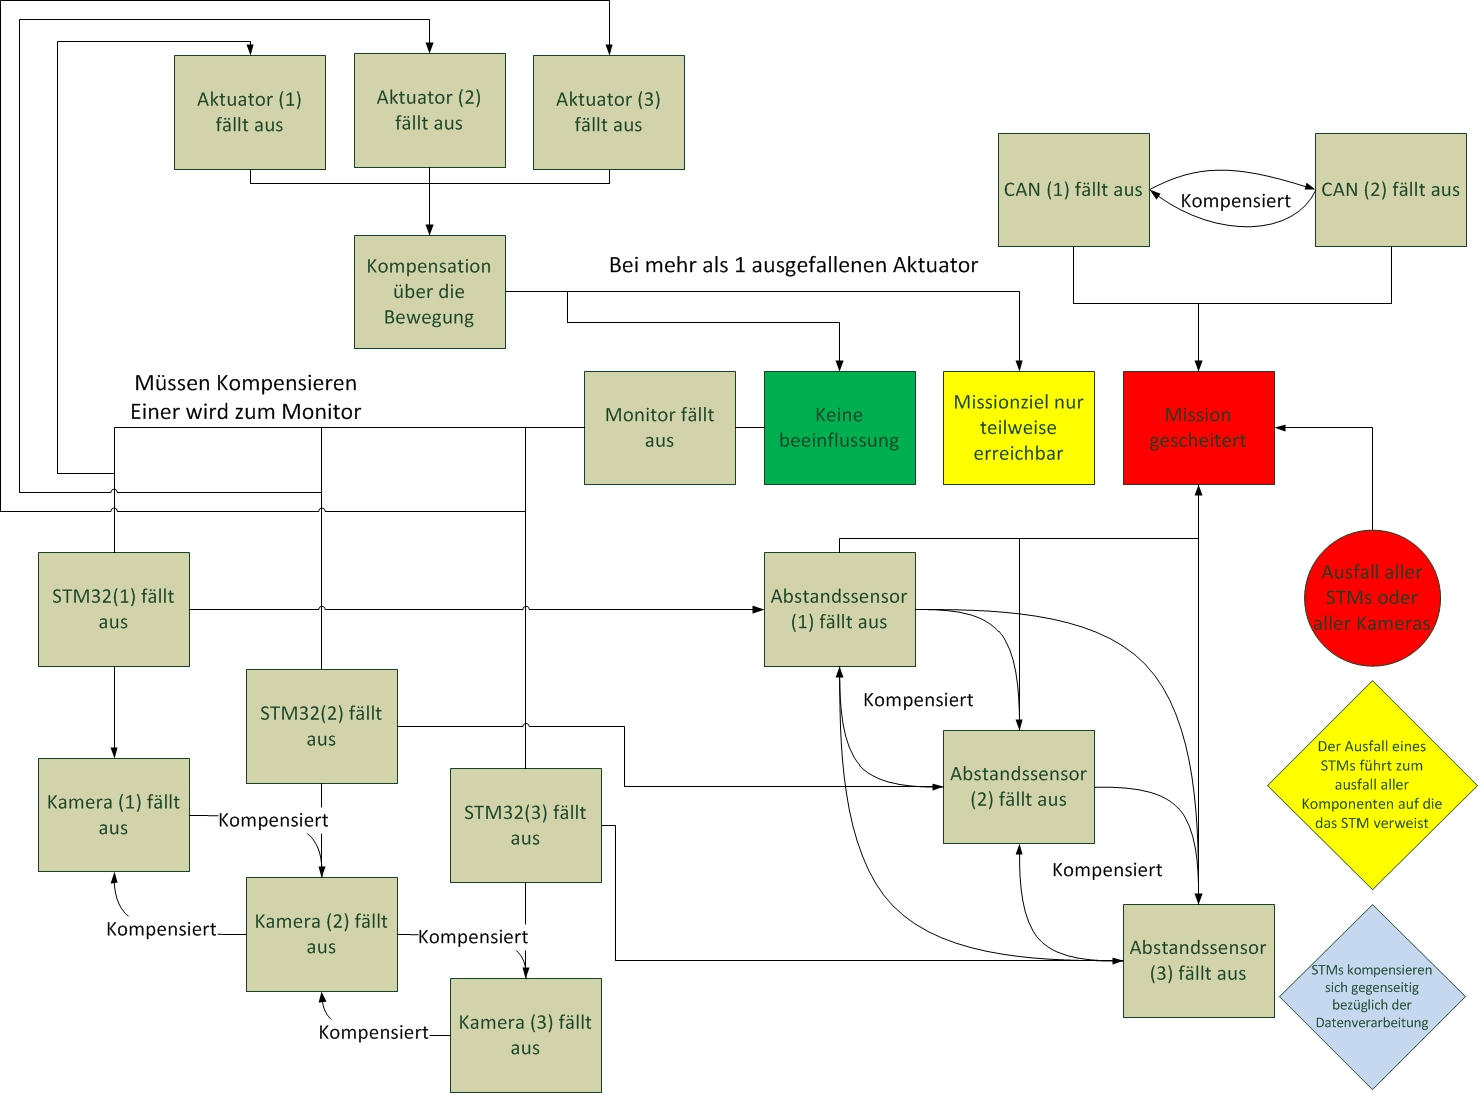
\includegraphics[width=\linewidth]{Bilder/FaTNet_fehlerverhalten}
\caption{Mögliche Fehlerfälle und entsprechende Kompensation}
\label{fig:fehlerverhalten}
\end{figure}

Bild \ref{fig:fehlerverhalten} veranschaulicht die verschiedenen Fehlerfälle, sowie die Möglichkeiten zu deren Kompensation grafisch.
Oben links in der Grafik wird gezeigt wie der Ausfall von Motoren am  Aktuator kompensiert wird.\\
Oben rechts sind die beiden CAN-Busse abgebildet, die ihren Ausfall wechselseitig kompensieren können.\\
Unten wird veranschaulicht, das System auf den Ausfall von STMs reagiert
Aus dem Systementwurf ergibt sich eine Ausfalltoleranz gegenüber bis zu zwei STMs, die Rechnungen bzw. die Steuerung wird dann  auf den/ die verbleibenden STM(s) ausgelagert um den Betrieb (unter Performanceeinbußen) fortzusetzen.\\
Da ein System nicht gegen jeden Komponentenausfall redundant sein kann, folgt eine Auflistung der konkreten Fehlerfälle mit denen das System umgehen kann. Alle Systemkomponenten, die nicht aufgelistet worden sind, wie z. B. die Antriebsmotoren und elektrischen Schaltungen und Leitungen, werden als \textit{Single Point of Failure} behandelt und sind nicht in der oberen Darstellung visualisiert. Das bedeutet, dass das System dann nicht in der Lage ist den Fehler zu finden und zu kompensieren.
Bild \ref{fig:fehlerverhalten} veranschaulicht die verschiedenen Fehlerfälle, sowie die Möglichkeiten zu deren Kompensation grafisch.


\paragraph{\textbf{Fehler 1: Ein STM fällt aus (siehe Abb. 8)}}$\;$\\
Das System verliert einen Aktuator, ein Abstandssensor sowie eine Kamera und abhängig vom ausgefallenen STM den Monitor.
Der fehlenden Aktuator reduziert den Freiheitsgrad des Manipulators, dadurch kann das Missionsziel bei mehr als einem ausgefallenen Aktuator nur noch teilweise erreicht werden. Der fehlende Freiheitsgrad kann durch das manövrieren des Demonstrators teilweise ausgeglichen werden, die ausgefallenen Abstandssensoren und Kameras wiederum schränken die Erfüllung des Missionsziels nicht ein, da diese redundant vorhanden sind.
Falls das ausgefallene STM in diesem Moment die Monitorfunktion übernahm, muss eines der verbliebenen STMs die Monitorfunktion übernehmen.

\begin{figure}[H]
\centering
  \begin{minipage}[b]{0.49\linewidth}
    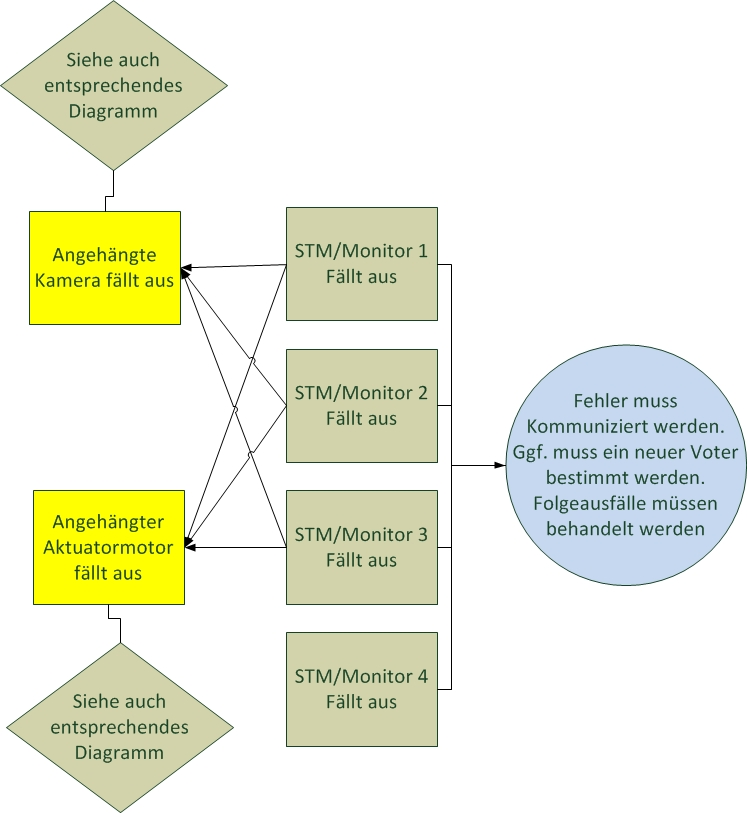
\includegraphics[width=\linewidth]{Bilder/FaTNet_stmredundanz} 
    \caption{Ausfall eines STM-Boards}
    \label{fig:stmredundanz}
  \end{minipage}
  \begin{minipage}[b]{0.49\linewidth}
    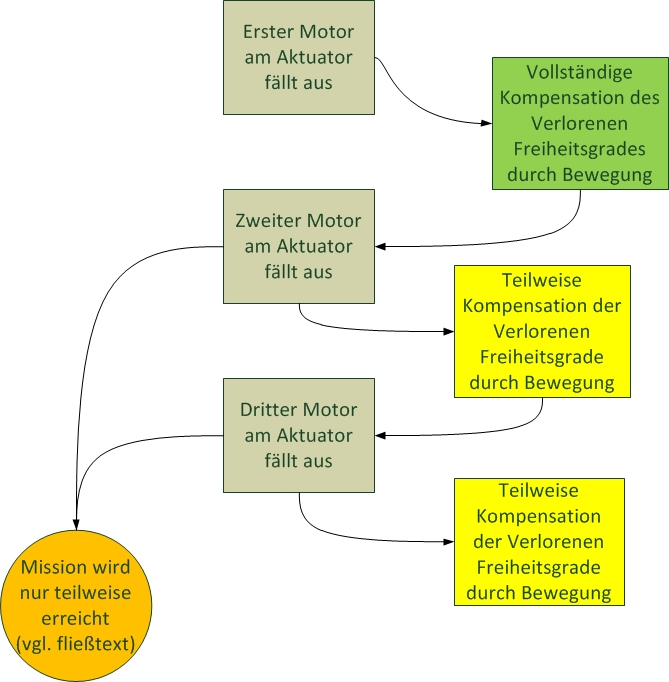
\includegraphics[width=\linewidth]{Bilder/FaTNet_aktuatorredundanz}  
    \caption{Ausfall eines  Aktuators}
    \label{fig:aktuatorredundanz}
  \end{minipage}
\end{figure}


\paragraph{\textbf{Fehler 2: Motor am Manipulator fällt aus (siehe Abb. 9)}}$\;$\\ 
Wie im Fehlerfall 1 kann das System den Verlust durch bewegen des Gesamtsystems teilweise kompensieren.
Wird ein ausgefallener Freiheitsgrad kompensiert ist der Manipulator immer noch in der Lage jede Raumposition anzufahren. Müssen zwei oder mehr ausgefallene Freiheitsgrade kompensiert werden kann es sein, dass der Manipulator nur eingeschränkte Raumpositionen anfahren kann. Dadurch kann das Missionsziel nur noch angenähert werden. Das System muss unter diesen Umständen das Ziel so gut es geht erreichen.

\paragraph{\textbf{Fehler 3: Monitor fällt aus (siehe Abb. 8)}}$\;$\\
Einer der anderen STMs übernimmt die Aufgabe des STM der vorher die Monitoraufgabe erfüllt hat, dadurch bleibt des Systems weiterhin voll funktionsfähig.
Die STMs sind intern durchnummeriert, das "ubriggebliebene STM mit der h"ochsten Nummer "ubernimmt die Funktion des Monitors.\\
Der Ablauf ist im Rahmen der STM-Redundanz erklärt.

\paragraph{\textbf{Fehler 4: Kamera fällt aus (siehe Abb. 10)}}$\;$\\
Es sind zwei Fehlerfälle möglich, zum Einen kann die Stromversorgung ausfallen, zum Anderen sendet die Kamera fehlerhafte Daten.
Falls die Stromversorgung für die Kamera ausfällt, übernehmen die redundanten Kameras die Funktion der ausgefallenen Kamera, dadurch bleibt das Missionsziel erreichbar.
Dieser Fehler wird dadurch erkannt das eine Kamera keine Daten mehr sendet.\\
Der zweite Fehlerfall, das senden falscher Daten, wird durch den Monitor kompensiert, d.h. der Monitor vergleicht die errechneten Daten und filtert die falschen Daten heraus.

\begin{figure}[H]
\centering
  \begin{minipage}[b]{0.49\linewidth}
    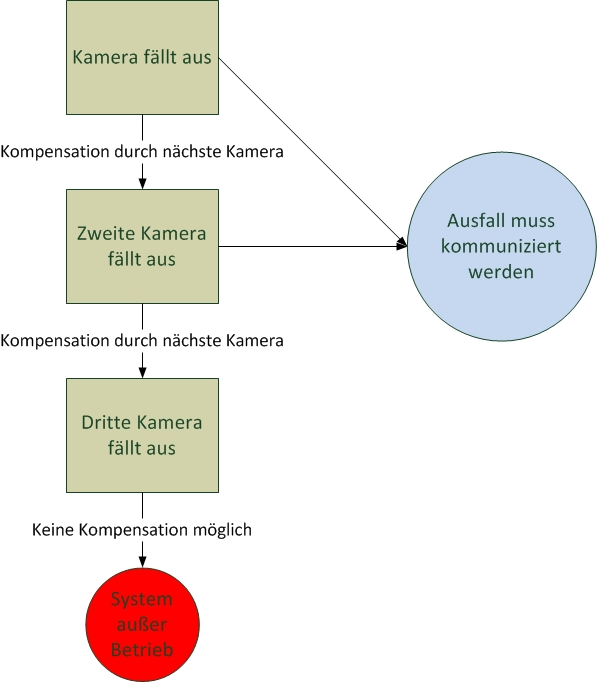
\includegraphics[width=\linewidth]{Bilder/FaTNet_kameraredundanz} 
    \caption{Ausfall einer Kamera}
    \label{fig:kameraredundanz}
  \end{minipage}
  \begin{minipage}[b]{0.49\linewidth}
    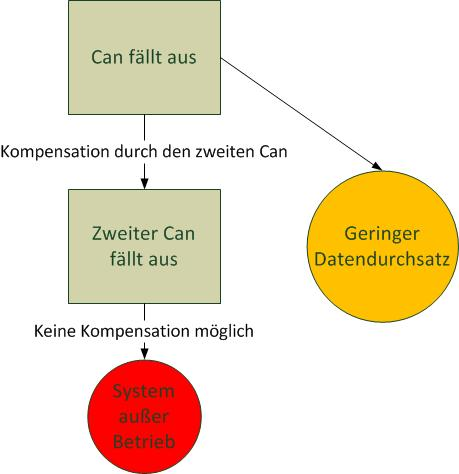
\includegraphics[width=\linewidth]{Bilder/FaTNet_canredundanz}  
    \caption{Ausfall eines CAN-Bus}
    \label{fig:canredundanz}
  \end{minipage}
\end{figure}

\paragraph{\textbf{Fehler 5: CAN-Bus fällt aus (siehe Abb. 11)}}$\;$\\
Der redundante CAN-Bus übernimmt die Aufgabe des ausgefallenen CAN-Bus, dadurch bleibt das System funktionsfähig.
Beim Ausfall des redundanten CAN-Bus ist keine weitere Kompensation mehr möglich und dementsprechend fällt das System aus.

\paragraph{\textbf{Fehler 6: Abstandssensor fällt aus (siehe Abb. 12)}}$\;$\\
Die redundanten Abstandssensoren übernehmen die Funktion der ausgefallenen Sensoren.
Der Ausfall eines Sensors wird dadurch ermittelt, dass dieser keine Daten mehr sendet.
\begin{figure}[H]
\centering
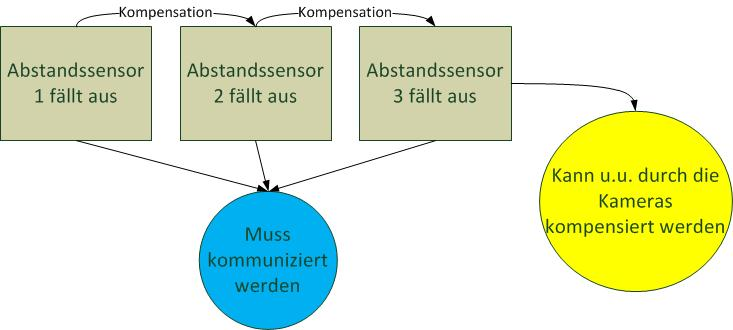
\includegraphics[width=0.7\linewidth]{Bilder/FaTNet_abstandssensoredundanz}
\caption{Ausfall eines Abstandssensors}
\label{fig:abstandssensorredundanz}
\end{figure}

\section{Testläufe}
\label{Testlaeufe}
Die folgenden Testfälle müssen durchgeführt werden um die Fehlertoleranz des Systems vollständig aufzuzeigen.
\begin{table}[H]
\centering
\begin{tabular}{|c|p{9cm}|p{5.5cm}|}
\hline 
Testlauf & Szenario (Ausfall) & Zielerfüllung\\ 
\hline
1 & Fehlerfreier Fall & vollständig\\ 
\hline 
2 & 1 Can + 1 Abstandssensor & vollständig\\ 
\hline 
3 & 1 Can + 1 Abstandssensor + 1 Aktuator & vollständig durch Kompensation\\ 
\hline 
4 & 1 Can + 1 Abstandssensor + 1 Aktuator + 1 Kamera & vollständig durch Kompensation\\ 
\hline 
5 & 1 Can + 1 Abstandssensor + 1 Aktuator(1) + STM(1) + 1 Kamera (2 oder 3) & vollständig durch Kompensation\\ 
\hline 
6 & 1 Can + 1 Abstandssensor + 1 Aktuator(1) + STM(1) + 1 Kamera (2 oder 3) + Voter & vollständig durch Kompensation\\ 
\hline 
7 & 1 Can + 1 Abstandssensor + 2 Aktuator(1 und 2) + 2 STM(1 und 2) + Kamera (2) + Voter & teilweise durch Kompensation\\ 
\hline 
8 & 1 Can + 1 Abstandssensor + 2 Aktuator(1 und 2) + 2 STM(1 und 2) + Kamera (2) + Voter + [Kamera(3) oder Aktuator(3) oder STM(3) oder CAN(2)] & Fehler\\ 
\hline 
\hline 
\end{tabular} 
\caption{Durchzuführende Testfälle}
\label{tab:testlaeufe}
\end{table}
Durch diese Testläufe wird die größtmögliche Verzahnung der verschiedenen Fehler erreicht, so dass der Roboter noch funktioniert. Die Fehler sind dabei so gewählt, dass erst zum Schluss kritische Zustände erreicht werden und im Laufe der Tests sichtbar wird, dass das System an Leistung verliert (Prinzip der Graceful degredation).\\
Die Tabelle 2 zeigt in Kombination mit Abbildung 7 das alle Funktionalit"aten bez"uglich der Redundanz des Systems aufgezeigt werden.\\
Die triviale Funktion des Systems wird im Fehlerfreien Fall gezeigt.
\section{Arbeitspakete und Zeitplanung}
\label{ArbeitspaketeUndZeitplanung}
Die genaue Arbeitsplanung ist im Diagramm \ref{fig:arbeitsablauf} im \nameref{kap:Anhang} zu finden.
Hier sind die Pakete allgemein bennant aber nicht beschrieben oder nach zeitlichem Ablauf sortiert.\\
\subsection{Hardware}
\begin{itemize}
	\item Bestellung
	\item Aktuator entwerfen und bauen
	\begin{itemize}
		\item Komponenten auswählen
		 \item Montieren
	\end{itemize}
	\item Chassis entwerfen und bauen
	\begin{itemize}
		\item Komponenten auswählen
		\item Montieren
	\end{itemize}
	\item Elektronik planen
	\begin{itemize}
		\item Kabelführung/Fehlerinjektion
		\item Stromversorgung der einzelnen Komponenten
		\item andere Elektronik
	\end{itemize}
	\item Sensorik
	\begin{itemize}
		\item auswählen und an geeigneter Stelle einbauen
	\end{itemize}
\end{itemize} 

\subsection{Software}
\begin{itemize}
	\item CAN Treiber/Protokoll
	\begin{itemize}
		\item Redundanz des Busses implementieren
	\end{itemize}
	\item Voter Funktion implementieren
	\item Treiber Aktuator
	\item Treiber Antrieb
	\item Treiber Kamera
	\item Treiber Abstandssensoren
	\item Bildverarbeitung
	\begin{itemize}
		\item Zielfindung
	\end{itemize}
	\item Navigation
	\item inverse Kinematik
	\begin{itemize}
		\item Kinematik berechnen
	\end{itemize}
	\item MUX implementieren
\end{itemize}


\subsection{Milestones}

\subsubsection{Hardware}
\begin{itemize}
	\item August 2013 Abschlusspräsentation
	\item April 2013 vollständiger Ausgang der Hardwarebestellung
	\item Juni 2013 abgeschlossener Hardwareaufbau
	\end{itemize}


\subsubsection{Software}
	Navigation:
\begin{itemize}
	\item Mai 2013 Bildverarbeitung
	\begin{itemize}
		\item Positionserkennung
		\item Voting
	\end{itemize}
	\end{itemize}


\section{Risikomanagement}
\label{Risikomanagement}
\subsection{Mögliche Schwierigkeiten}
\subsubsection{Ausfall von (bereits verbauten) Systemkomponenten}
Sollten Teile der Bestellung bei Lieferung beschädigt sein, oder im Laufe des Einbaus oder der Arbeit mit ihnen funktionsunfähig werden, so kann dies zu einiger Verzögerung im Projektablauf führen. Die Komponenten müssen ggf. wieder ausgebaut werden, sofern möglich repariert und ansonsten neubestellt werden. Je nachdem welches Teil ausfällt, kann nicht nur der endgültige Aufbau der Hardware dadurch verzögert werden, sondern auch das Testen bestimmter Funktionalitäten.

\subsubsection{Kinematik des Manipulators bei Stromausfall}
Bisher ist noch ungeklärt, wie sich der Manipulator bei Stromausfall der Aktuatoren verhält. Möglicherweise bleiben die Gelenke steif, eventuell sinkt der Arm aber auch in sich zusammen. Sollte letzteres eintreffen, müssen geeignete Gegenmaßnahmen gefunden und angewendet werden, damit eine eingeschränkte Bewegungsfähigkeit erhalten bleibt (siehe Kaptiel \ref{kap:Manipulator}: \nameref{kap:Manipulator}).

\subsubsection{Umgang mit Komplikationen}
Sollte aus oben genannten Gründen, oder anderen unvorhersehbaren Komplikationen eine Verzögerung in der  Projektdurchführung resultieren, so können folgende Maßnahmen ergriffen werden, um einen erfolgreichen Projektabschluss zu gewährleisten.

\subsubsection{Monitor wird zum Single Point of Failure}
Im Projektentwurf ist vorgesehen, dass bei Ausfall des Voters eines der anderen STMs dessen Rolle übernimmt. Die diesbezügliche Fehlertoleranz könnte im Zweifelsfall aufgegeben werden und der Voter stattdessen als Single Point of Failure behandelt werden.

\subsubsection{CAN-Bus wird zum Single Point of Failure}
Es ist vorgesehen den CAN-Bus redundant anzulegen. Sollte es dabei jedoch zu Problemen kommen, kann dieser zum Single Point of Failure vereinfacht werden.
\section{Anhang}
\label{kap:Anhang}
\clearpage
\setlength\pdfpagewidth{600mm}
\setlength\pdfpageheight{600mm}
\begin{figure}[p]
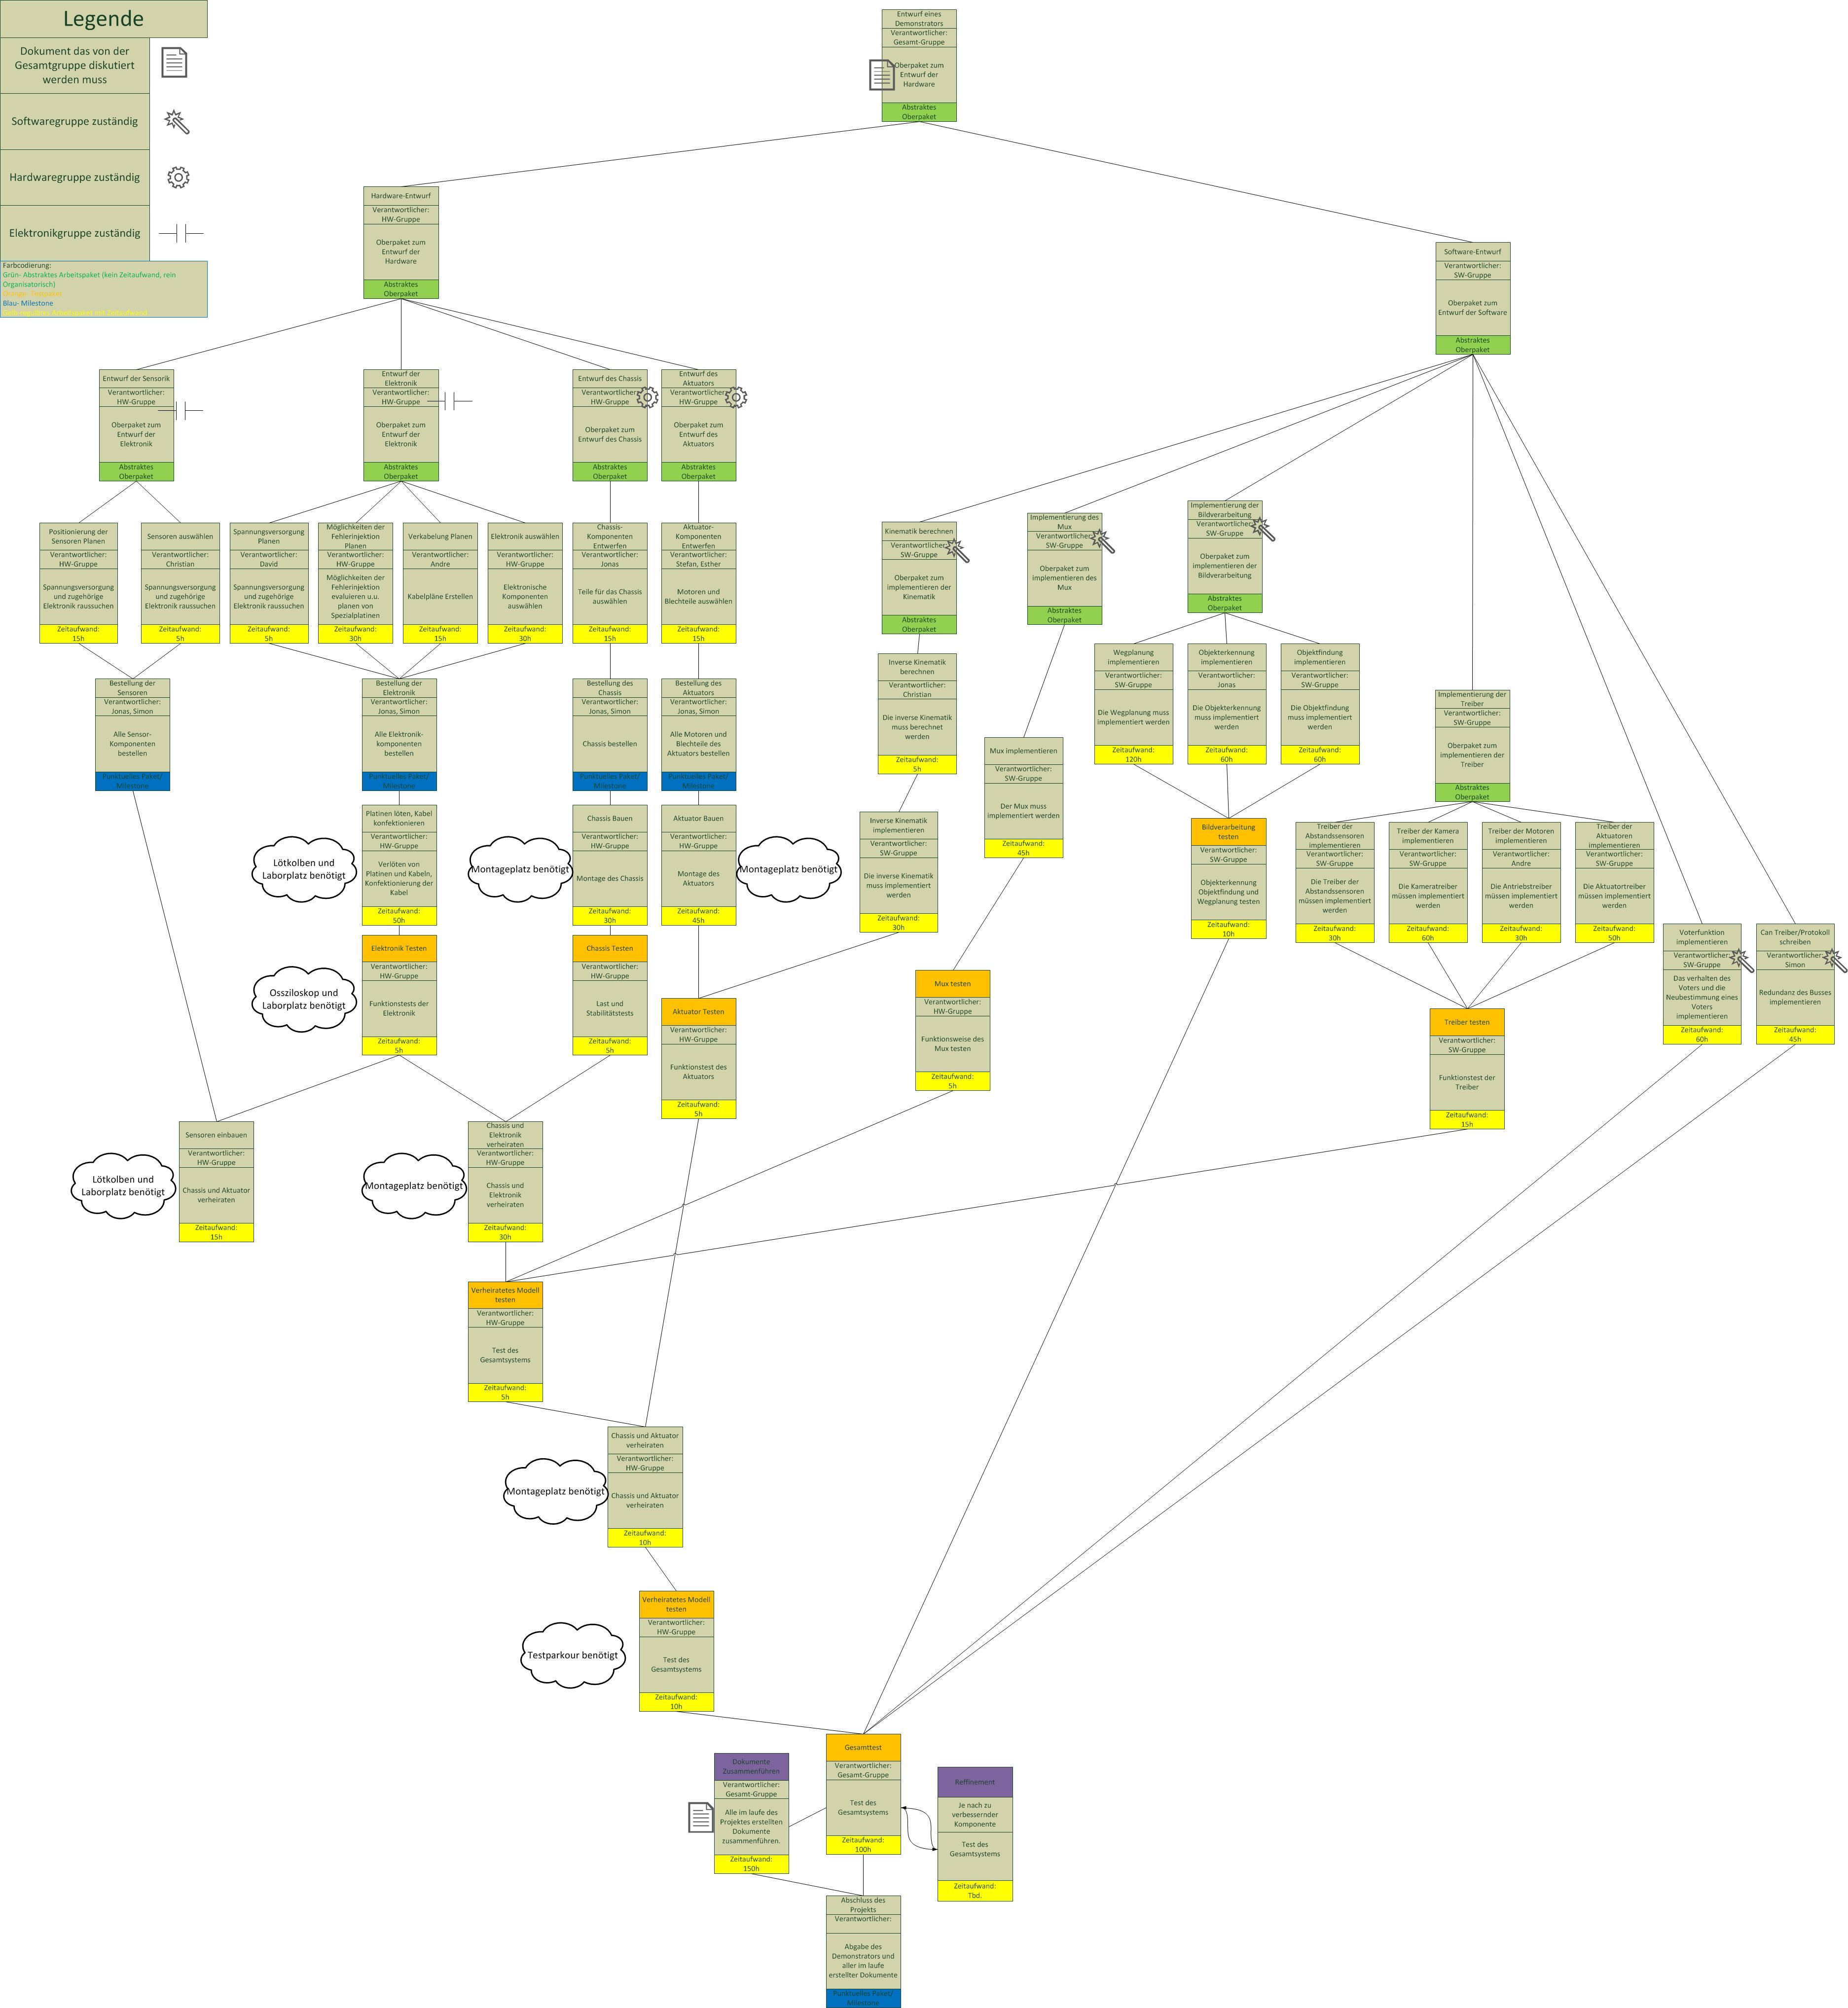
\includegraphics[height=500mm]{Bilder/FaTNet_arbeitsablauf}
\caption{Geplanter Arbeitsablauf}
\label{fig:arbeitsablauf}
\end{figure}

\clearpage

\setlength\pdfpagewidth{210mm}
\setlength\pdfpageheight{297mm}

\end{document}
